


\section{Problem 1}
\label{part1}

Demonstrate that you know how to use "curl" well enough to
correctly POST data to a form.  Show that the HTML response that
is returned is "correct".  That is, the server should take the
arguments you Posted and build a response accordingly.  Save the
HTML response to a file and then view that file in a browser and
take a screen shot.

\subsection{Solution}

\begin{enumerate}
	\item Started with understanding what curl does from the secure shell by using curl --help command.
	\item Got various options which are used in curl. Later,Referred few sites in order to get in touch with curl.
	\item My next step was to get the web forms which use POST method but It was hard to find them. Later, I found the link in the goggle groups and started using it.
	\item I selected the following web page to post my data.
\begin{verbatim}
	http://www.cs.tut.fi/cgi-bin/run/~jkorpela/echo.cgi 	
\end{verbatim}
	\item The curl command i used to post data to a form is 
\begin{verbatim}
	Curl --data "comments=Good to see you" 
	http://www.cs.tut.fi/cgi-bin/run/~jkorpela/echo.cgi -o output.html
\end{verbatim}
	\item In the beginning i did not use -o output.html and so i got the html code as output on my command prompt.
	\item curl -o output.html command creates a html file in the Z drive.  
\end{enumerate}
\newpage
\subsection{Results}
\begin{enumerate}
 	\item Screen shot of the web page with the form to which I posted data is shown below.
\begin{figure}[ht]    
    \begin{center}
        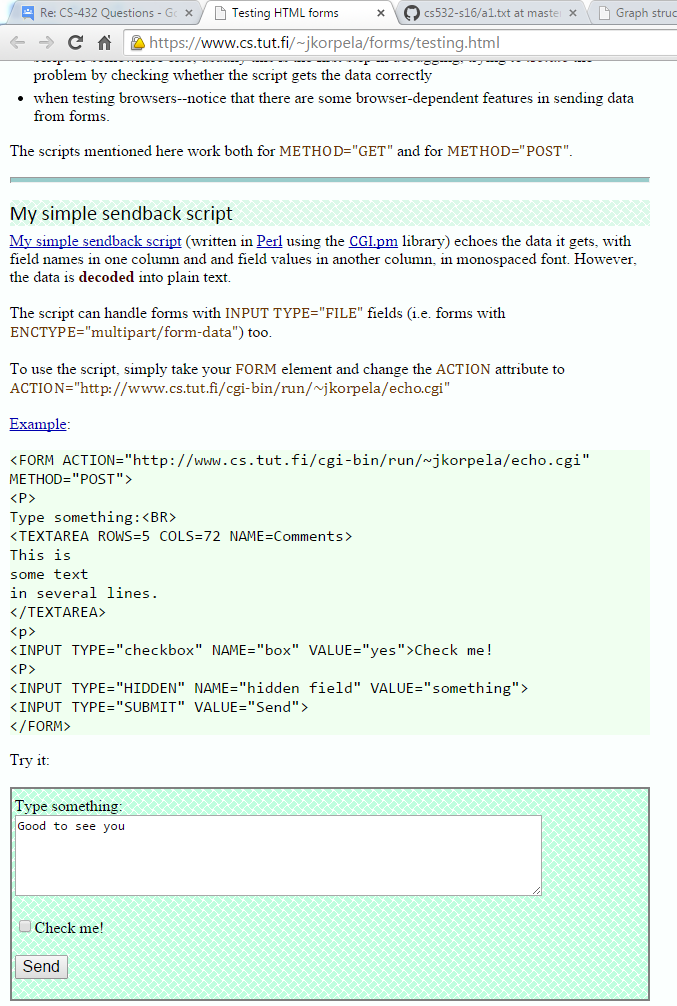
\includegraphics[scale=0.60]{Form_in_webpage.png}
        \caption{Form in the Web page}
        \label{fig:X-distribution}
    \end{center}
\end{figure}
\newpage
	\item The response I got after implementing the curl command is shown below

\begin{figure}[ht]    
    \begin{center}
        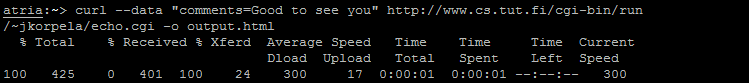
\includegraphics[scale=0.90]{Cmd_line_response.png}
        \caption{Response for the curl command}
        \label{fig:X-distribution}
    \end{center}
\end{figure}

	\item Screen shot of the html file in the browser is shown below.

\begin{figure}[ht]    
    \begin{center}
        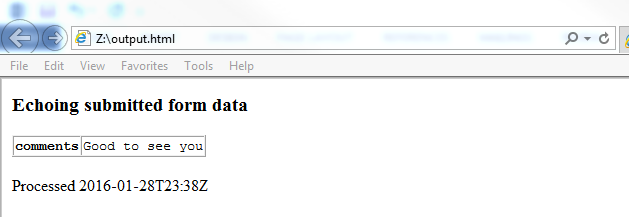
\includegraphics[scale=0.90]{Response_from_browser.png}
        \caption{Response from the browser}
        \label{fig:X-distribution}
    \end{center}
\end{figure}
\end{enumerate}
